\documentclass{BHCexam}	
\begin{document}
\begin{questions}
\qs 在三角形$\triangle ABC$中,$ \angle BAD=30^{\circ},\angle CAD=45^{\circ},~AB=2,~AC=2 $则$ \dfrac{BD}{DC}= $\tk.
\vspace{-2em}
\begin{center}
\begin{tikzpicture}[line width=0.7 pt,scale=0.7]
%\draw[help lines] (0,0) grid (4,3);
\coordinate[label=below:\small$B$](B) at (0,0);
\coordinate[label=below:\small$C$](C) at(3,0);
\coordinate [label=above:\small$A$](A) at(2,2);
\coordinate [label=below:\small$D$](D) at ($(B)!0.4!(C)$);
\draw (B)--(A)--(C)--cycle (A)--(D);
\end{tikzpicture}
\end{center} 
\qs 已知函数$f(x)=\Bigg\{\begin{aligned}
\sin(x+\alpha),x\le 0\\\cos (x+\alpha),x>0
\end{aligned}$则“$ \alpha=\dfrac{\pi}{4} $”是“函数$f(x)$是偶函数”的\xx
\twoch{充分不必要条件}{必要不充分条件}{充分必要条件}{既不充分也不必要条件}
\qs 已知函数$f(x)=\Bigg\{\begin{aligned}
\sin(x+a),x\le 0\\\cos (x+b),x>0
\end{aligned}$是偶函数,则下列结论可能成立的是\xx
\twoch{$ a=\dfrac{\pi}{4},b=-\dfrac{\pi}{4}$}{$ a=\dfrac{2\pi}{3},b=\dfrac{\pi}{6}$}{$a=\dfrac{\pi}{3},b=\dfrac{\pi}{6} $}{$ a=\dfrac{5\pi}{6},b=\dfrac{2\pi}{3}$}
\qs 已知函数$f(x)=\sin (\omega x-\dfrac{\pi}{3})$,~点$ A(m,n) $,~$ B(m+\pi,n) (\left|n\right|\ne 1)$都在曲线$ y=f(x) $上,且线段$ AB $与曲线$ y=f(x) $有五个公共点,则$ \omega $的值为\xx
\onech{$ 4 $}{$ 2 $}{$ \dfrac{1}{2} $}{$ \dfrac{1}{4} $}
\qs 在$\triangle ABC$中,角$ A,B,C $所对的边分别是$ a,\ b,\ c $,且$ a,\ b,\ c $成等差数列,则角$ B $的取值范围是\xx
\onech{$ \left(0,\dfrac{\pi}{3}\right]$}{$ \left(\dfrac{\pi}{6},\dfrac{\pi}{2}\right)$}{$ \left(\dfrac{\pi}{4},\dfrac{\pi}{2}\right)$}{$ \left(\dfrac{\pi}{3},\dfrac{\pi}{2}\right)$}
\qs 已知函数$f(x)=\sin (2x+\varphi)$,若$ f(\dfrac{\pi}{12})-f(\dfrac{-5\pi}{12})=2 $,则函数$f(x)$的单调增区间为\tk.
\qs 已知函数$ y=2\sin\left(\omega x+\varphi\right) \left(w>0,\abs{\varphi}<\dfrac{\pi}{2}\right)$.\\
\ding{192}若$f(0)=1$,则$ \varphi= $\tk;\\
\ding{193}若$ \exists x\inR $,使$ f(x+2)-f(x)=4 $成立,则$ \omega  $的最小值为\tk.





\newpage
\qs 如图,在四边形$ ACBD $中,$ \cos\angle CAD=-\dfrac{1}{7} $,且$ \triangle ABC $为正三角形.
\begin{parts}
	\part 求$ \cos \angle BAD $的值;
	\part 若$ CD=4,BD=\sqrt{3} $,求$ AB $和$ AD $的长.
\end{parts}
\vspace{-5em}
\mbox{\hspace{1em}}\hfill 
	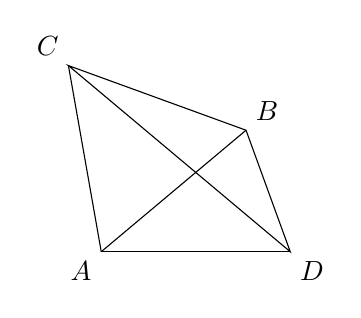
\begin{tikzpicture}[scale=0.6]
	\draw(0,0)node[coordinate,label=below left:$A$](A){$A$}--(4,0)node[coordinate,label=below right:$D$](D){$D$};
	\draw (A)--+(40:4)node[coordinate,label=above right:$B$](B){$B$};
	\draw (A)--(100:4)node[coordinate,label=above left:$C$](C){$ $};
	\draw (C)--(B)--(D)--cycle;
	
	\end{tikzpicture}

\kongbai 

\qs 已知函数$f(x)=-2\sin x-\cos 2x$.
\begin{parts}
\part 比较$ f(\dfrac{\pi}{4}) ,~f(\dfrac{\pi}{6})$的大小;
\part 求函数$f(x)$的最大值.
\end{parts}
\kongbai
\qs 在锐角$\triangle ABC$中,角$ A,B,C $所对的边分别为$ a,b,c $,已知$ a=\sqrt{7},~b=3,~\sqrt{7}\sin B+\sin A=2\sqrt{3}.$
\begin{parts}
\part 求角$ A $的大小;
\part 求$\triangle ABC$的面积
\end{parts}
\kongbai
\qs 在三角形$\triangle ABC$中,角$ A,~B,~C $所对的边分别为$ a,~b,~c $,且$ \sin^2 A=\sin B\sin C $.
\begin{parts}
\part 若$ \angle A=\dfrac{\pi}{3},~ $求$ \angle B $的大小;
\part 若$ bc=1, ~$求$\triangle ABC$的面积的最大值.
\end{parts}
\kongbai
\qs 如图,在三角形$\triangle ABC$中,$ \angle ABC=90^{\circ} ,AB=4,BC=3,~$点$ D $在线段$ AC $上,且$ AD=4DC $.
\begin{parts}
\part 求$ BD $的长;
\part 求$ \sin CBD $的值.
\end{parts}
\mbox{\hspace{1em}}\hfill
\begin{tikzpicture}[line width=0.7 pt,scale=0.7]
%\draw[help lines] (0,0) grid (4,3);
\coordinate[label=left:$B$](B) at (0,0);
\coordinate[label=right:$C$](C) at(3,0);
\coordinate [label=above:$A$](A) at(0,4);
\coordinate [label=right:$D$](D) at ($(A)!0.75!(C)$);
\draw (B)--(A)--(C)--cycle (B)--(D);
\end{tikzpicture}
\kongbai
\vspace{-7em}
\qs 已知函数$f(x)=(1+\sqrt{3}\tan x)\cos^2x .$
\begin{parts}
\part 若$ \alpha $是第二象限角,且$ \sin \alpha=\dfrac{\sqrt{6}}{3} $,求$ f(\alpha) $的值;
\part 求函数$f(x)$的定义域和值域. 
\end{parts}
\kongbai
\qs 在三角形$\triangle ABC$中,角$ A,~B,~C $所对的边分别为$ a,~b,~c ,~$已知$ b^2+c^2=a^2+bc. $
\begin{parts}
\part 求$ A $的大小;
\part 如果$ \cos B=\dfrac{\sqrt{6}}{3},b=2 ,~$求三角形$\triangle ABC$的面积.
\end{parts}
\kongbai
\qs 已知函数$f(x)=2\sin \dfrac{\pi}{6}x\cos \dfrac{\pi}{6}x,~$过两点$ A\left(t,f(t)\right) ,~B\left(t+1,f(t+1)\right)$的直线的斜率记为$ g(t). $
\begin{parts}
\part 求$ g(0) $的值;
\part 写出函数$ g(t) $的解析式,求$ g(t) $在$ \left[-\dfrac{3}{2},\dfrac{3}{2}\right] $上的取值范围.
\end{parts}
\kongbai
\qs 已知函数$f(x)=\sin \omega x(\cos \omega x-\sqrt{3}\sin \omega x)+\dfrac{\sqrt{3}}{2}~(\omega >0)$的最小正周期为$ \dfrac{\pi}{2}. $
\begin{parts}
\part 求$ \omega $的值;
\part 求函数$f(x)$的单调递减区间.
\end{parts}
\kongbai
\qs 如图,在三角形$\triangle ABC$中,点$ D $在边$ AB $上,且$ \dfrac{AD}{DB} =\dfrac{1}{3}$.~记$ \angle ACD=\alpha~\angle BCD=\beta. $
\begin{parts}
\part 求证:$ \dfrac{AC}{BC}=\dfrac{\sin \beta }{3\sin \alpha} $;
\part 若$ \alpha=\dfrac{\pi}{6},~AB=\sqrt{19},~ $求$ BC $的长.
\end{parts}
\vspace{-5em}\mbox{\hspace{1pt}}\hfill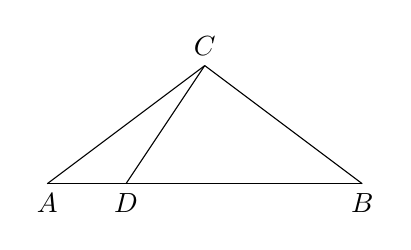
\begin{tikzpicture}
\coordinate [label=below:$A$](A) at (0,0);
\coordinate[label=below:$D$](D) at(1,0);
\coordinate[label=below:$B$](B) at(4,0);
\coordinate[label=above:$C$](C) at(2,1.5);
\foreach \p in{A,B,D}
\draw (C)--(\p);
\draw (A)--(B);
\end{tikzpicture}
\kongbai
\qs 已知函数$f(x)=\sin^2\left(x+\dfrac{\pi}{4}\right)$.
\begin{parts}
\part 求$f(x)$的最小正周期及其图象的对称轴方程;
\part 求$ f\left(\dfrac{\pi}{3}-x\right) $的单调递减区间.
\end{parts}
\end{questions}
\end{document}